\documentclass[a4paper,8pt]{article}
\usepackage[utf8]{inputenc}
\usepackage[top=0.75in, bottom=0.75in, left=0.55in, right=0.85in]{geometry}
\usepackage{graphicx}
\usepackage{palatino}
\usepackage{tabularx}
\usepackage{enumitem}
\geometry{textwidth=7cm}
\newlength{\outerbordwidth}
\pagestyle{empty}
\raggedbottom
\raggedright
%\graphicspath{{F:\Important_Documents\Uploaded}}
\usepackage[svgnames]{xcolor}
\usepackage{framed}
\usepackage{tocloft}
\definecolor{mygrey}{gray}{0.55}
\setlength{\outerbordwidth}{3pt}  % Width of border outside of title bars
\setlength{\evensidemargin}{-0.25in}
\setlength{\headheight}{0in}
\setlength{\headsep}{0in}
\setlength{\oddsidemargin}{-0.25in}
\setlength{\paperheight}{11in}
\setlength{\paperwidth}{8.5in}
\setlength{\tabcolsep}{0in}
\setlength{\textheight}{9.5in}
\setlength{\textwidth}{7in}
\setlength{\topmargin}{-0.3in}
\setlength{\topskip}{0in}
\setlength{\voffset}{0.1in}
\setlist{leftmargin=3.28mm}
\renewcommand*\rmdefault{phv}
\newcommand{\resheading}[1]{{\normalsize \colorbox{mygrey}
{\begin{minipage}
{1\textwidth}{\textbf{\sffamily{\mbox{~}\makebox[5.9in][l]{\large #1} \vphantom{p\^{E}}}}}
\end{minipage}}}}


\newgeometry{left=0.35in,right=0.35in,top=0.25in,bottom=0.25in}
%%%%%%%%%%%%%%%%%%%%%%%%%%%%%%%%%%%%%%%%%%%%%%%%%%%%%%%%%%%%%%%%%%%%%%
%%%%%%%%%%%%%%%%%%%%        TITLE          %%%%%%%%%%%%%%%%%%%%%%%%%%%
\begin{document}
\begin{tabular*}{7.6in}{l@{\extracolsep{\fill}}r}
{\Huge R\huge OMIL \Huge K\huge ADIA} & {\textit{romil@iitk.ac.in} $\mid$ +91-942-912-0451} \\
\end{tabular*}
\\
%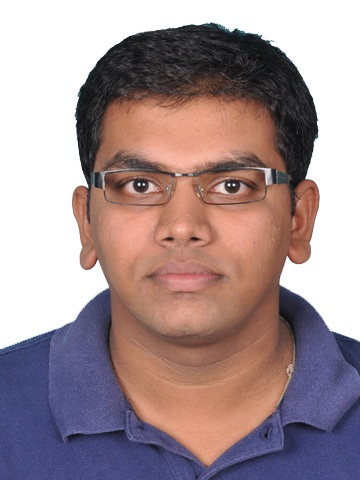
\includegraphics[scale=1.5]{photo}
%%%%%%%%%%%%%%%%%%%%%%%%%%%%%%%%%%%%%%%%%%%%%%%%%%%%%%%%%%%%%%%%%%%
%%%%%%%%%%%%%%%%%%       TABULAR          %%%%%%%%%%%%%%%%%%%%%%%%%%%
\resheading{\color{white} \large A\normalsize CADEMIC \large D\normalsize ETAILS}
 \indent 
 \centering 
 \begin{tabular}{ l @{\hskip 0.58in} l @{\hskip 0.58in} l @{\hskip 0.59in} l @{\hskip 0.1in} l }
\hline
\textbf{Year} & \textbf{Qualification} & \textbf{Institute, City} & \textbf{CPI/\%} \\
\hline
2018 & M.Tech - Solid Mechanics and Design & Indian Institute of Technology Kanpur & 7.8/10\\
2015 & B.E. - Mechanical Engineering & Gujarat Technological University(LDRP-ITR) & 9.02/10\\
2011 & Intermediate/+2 (GSEB) & Amrut school, Ahmedabad & 83.33\%\\
2009 & Matriculation (GSEB) & Amrut school, Ahmedabad & 76.92\%\\
\end{tabular}
%%%%%%%%%%%%%%%%%%%%%%%%%%%%%%%%%%%%%%%%%%%%%%%%%%%%%%%%%%%%%%%%%%
%%%%%%%%%%%%%%%%%% KEY SCHOLATIC ACHIVEMENTS %%%%%%%%%%%%%%%%%%%%%
%%%%%%%%%%%%%%%%%%%%%%%%%%%%%%%%%%%%%%%%%%%%%%%%%%%%%%%%%%%%%%%%%%
\resheading{\color{white} \large K\normalsize EY \large S\normalsize CHOLASTIC \large A\normalsize CHIVEMENTS}
\begin{itemize}[topsep=0pt]
\setlength{\itemsep}{-3pt}
\item \makebox[\linewidth][s]{Ranked \textbf{1$^{st}$} in \textbf{Bachelor of Engineering} in Department of Mechanical Engineering at LDRP-ITR}
\item Awarded with \textbf{Institute Gold Medal} by Prof. Arvind R. Patel on behalf of Kadva Patidal Kelavni Mandal in 2015.
\item Secured \textbf{All India Rank 786} in \textbf{GATE, 2016} among 0.21 million mechanical engineering candidates.
\item Ranked \textbf{27$^{th}$} in Bachelor of Engineering in Mechanical engineering batch of 2015 at Gujarat Technological University.
\item Conferred with \textbf{Maneklal M. Patel Memorial Scholarship} for academic year 2014-15 \textit{(given to top 1\% student from institute)} for their {excellent performance} at Kadi Sarva Vishwavidyalaya by President Vallabhbhai M. Patel.
\end{itemize}
%%%%%%%%%%%%%%%%%%%%%%%%%%%%%%%%%%%%%%%%%%%%%%%%%%%%%%%%%%%%%%%%%%%
%%%%%%%%%%%%%%%%% COMPUTER SKILLS %%%%%%%%%%%%%%%%%%%%%%%%%%%%%%
%%%%%%%%%%%%%%%%%%%%%%%%%%%%%%%%%%%%%%%%%%%%%%%%%%%%%%%%%%%%%%%%%%%
\resheading{\color{white} \large C\normalsize OMPUTER \large S\normalsize KILLS}
\begin{itemize}[topsep=0pt]
\setlength{\itemsep}{-3pt}
\item \textbf{Programming Language:} Python, C/C++, JAVA, HTML/CSS, Fortran-95, Scheme.
\item \textbf{Software:} Solidworks, ANSYS, ABAQUS, MatLab, LATEX, Tinker, AutoCAD, Creo-Parametric.
\end{itemize}
%%%%%%%%%%%%%%%%%%%%%%%%%%%%%%%%%%%%%%%%%%%%%%%%%%%%%%%%%%%%%%%%%%
%%%%%%%%%%%%%%%%%% COURSES UNDERTAKEN %%%%%%%%%%%%%%%%%%%%%%%%%%%%
%%%%%%%%%%%%%%%%%%%%%%%%%%%%%%%%%%%%%%%%%%%%%%%%%%%%%%%%%%%%%%%%%%
\resheading{\color{white} \large C\normalsize OURSES \large U\normalsize NDERTAKEN}
\begin{itemize}[topsep=0pt]
\setlength{\itemsep}{-3pt}
\item \textbf{Mechanical Engineering:} Strength of Material, Solid Mechanics, Molecular Dynamics Simulations, Finite Element Method (Linear, Non-linear), Vibration of Continuous Systems (1D,2D), Advance Dynamics.
\item \textbf{Computer Science and Engineering:} Machine Learning(CS771A, IITK(Audit)), Data Structure and Algorithm in JAVA(CS61B,UC Berkeley(online)), Structure and Interpretation of Computer Program(CS61B, UC Berkeley(online)), Introduction to Algorithms(6.006, MIT OCW), Computer system Engineering(6.033, MIT OCW), Operating System(CS140, Stanford(online)), Theory of Computation(6.045, MIT OCW).
\end{itemize}
%%%%%%%%%%%%%%%%%%%%%%%%%%%%%%%%%%%%%%%%%%%%%%%%%%%%%%%%%%%%%%%%%%%
%%%%%%%%%%%%%%%%% POR %%%%%%%%%%%%%%%%%%%%%%%%%%%%%%
%%%%%%%%%%%%%%%%%%%%%%%%%%%%%%%%%%%%%%%%%%%%%%%%%%%%%%%%%%%%%%%%%%%
\resheading{\color{white} \large S\normalsize TUDENT \large G\normalsize OVERNANCE}
\begin{tabular*}{7.6in}{l@{\extracolsep{\fill}}r}
\textbf{Department Placement Moderator (ME)} & \textbf{IIT Kanpur}\\
Student Placement Office & \textit{May'17-Present}
\end{tabular*}

\begin{itemize}[topsep=0pt]
\setlength{\itemsep}{-3pt}
\item Integral member of \textbf{3-tier team} of \textbf{120 members} to facilitate placements of \textbf{1200+} graduating students.
\item Developing and strengthening contact with \textbf{400+} core companies and inviting them for upcoming placement session.
\item Responsible for guiding and helping the mechanical engineering students in their placement preparation.
\end{itemize}
\hrule \vfill
%%%%%%%%%%%%%%%%%%%%%%%%%%%%%%%%%%%%%%%%%%%%%%%%%%%%%%%%
\begin{tabular*}{7.6in}{l@{\extracolsep{\fill}}r}
\textbf{Web Administrator} & \textbf{IIT Kanpur}\\
Association of Mechanical Engineers & \textit{July'17-Present}
\end{tabular*}
\begin{itemize}[topsep=0pt]
\setlength{\itemsep}{-3pt}
\item Carried out maintenance, planning of content and improved the online presence of IIT Kanpur’s AME website.
\item Connected \textbf{500+} students of mechanical engineering and officials as well as Professors through an informal mean
\item Started a web platform (\textbf{AME Digital Library}) to enable collaboration of academic literature among students.
\end{itemize}
%%%%%%%%%%%%%%%%%%%%%%%%%%%%%%%%%%%%%%%%%%%%%%%%%%%%%%%%%%%%%%%%%%%
%%%%%%%%%%%%%%%%% THESIS AND PROJECT %%%%%%%%%%%%%%%%%%%%%%%%%%%%%%
%%%%%%%%%%%%%%%%%%%%%%%%%%%%%%%%%%%%%%%%%%%%%%%%%%%%%%%%%%%%%%%%%%%
\resheading{\color{white} \large T\normalsize HESIS AND \large P\normalsize ROJECTS}
\begin{tabular*}{7.6in}{l@{\extracolsep{\fill}}r}
%%%%%%%%%%%%%%%%%%%%%%%%%%%%%%%%%%%%%%%%%%%%%%%%%%%%%%%%%%%%%%%%%%%%
\textbf{Study of Dislocation and Disclination Motion of Graphene at zero kelvin} & \textbf{M.Tech Thesis, IIT Kanpur}\\
\textit{MD Simulation}, Thesis Supervisors Dr. Anurag Gupta and Dr. Shakti Singh Gupta & \textit{Dec'16-present}
\end{tabular*}
\begin{itemize}[topsep=0pt]
\setlength{\itemsep}{-3pt}
\item Study of Diclocation and Disclination and their motion of \textbf{Fullerene, Torus, CNT, Graphene sheet (Plain and Hollow)}.
\item Analysis of each object was done by \textbf{Molecular Simulation (Tinker)} and for that input files were generated using \textbf{Python}.
\item Visualized defects and their energy variation was noted using \textbf{Force Field Explorer (FFE)} using \textbf{mm-3 (2000) potential}.
\item Developed network model of optimization using continuum approach on \textbf{Python, MATLAB} and \textbf{JAVA} to match MD results.
\item Concluded that \textbf{Defects are stable at central portion of structure} and they should match object's topology constraints.
\end{itemize}
\hrule \vfill
%%%%%%%%%%%%%%%%%%%%%%%%%%%%%%%%%%%%%%%%%%%%%%%%%%%%%%%%%%%%%%%%%%%
\begin{tabular*}{7.6in}{l@{\extracolsep{\fill}}r}
\textbf{Design and Development of Centrifugal Type Positive Frictional Clutch} & \textbf{B.E. Project, LDRP-ITR}\\
\textit{Automotive Engineering}, Project Supervisor Prof. D. H. Pandya & \textit{May'14-May'15}
\end{tabular*}
\begin{itemize}[topsep=0pt]
\setlength{\itemsep}{-3pt}
\item Avoided clutch slip phenomena by using the combination of centrifugal type, positive and frictional type disc clutch.
\item Generated model of complete system using \textbf{Solidworks} in first phase and analysis of each component and Assembly as well as sub-Assembly was done in second phase \textbf{ANSYS Static Structure toolbar}.
\item Patent has been filed and communication is going on with \textbf{Indian Patent Office} for design related issues.
\end{itemize}
\hrule \vfill
%%%%%%%%%%%%%%%%%%%%%%%%%%%%%%%%%%%%%%%%%%%%%%%%%%%%%%%%%%%%%%
\begin{tabular*}{7.6in}{l@{\extracolsep{\fill}}r}
\textbf{Symbol identification} & \textbf{Course Project, IIT Kanpur}\\
\textit{ML}, under guidance Dr. Purushottam Kar & \textit{Aug'17-Present}
\end{tabular*}
\begin{itemize}[topsep=0pt]
\setlength{\itemsep}{-3pt}
\item Given math/text symbols in handwritten form and that too as in combination, Machine gives LaTeX code for that symbol.
\end{itemize}
\hrule \vfill
%%%%%%%%%%%%%%%%%%%%%%%%%%%%%%%%%%%%%%%%%%%%%%%%%%%%%%%%%%%%%%%%
\begin{tabular*}{7.6in}{l@{\extracolsep{\fill}}r}
\textbf{Design of Scheme interpreter in CS61A} & \textbf{Course Project, UC Berkeley(online)}\\
\end{tabular*}
\begin{itemize}[topsep=0pt]
\setlength{\itemsep}{-3pt}
\item Developed an interpreter for a subset of the \textbf{Scheme} language using \textbf{Python}. The project concludes with an graphics challenge to produce recursive images in only a few lines of code in Scheme language.
\end{itemize}
%\pagebreak
%%%%%%%%%%%%%%%%%%%%%%%%%%%%%%%%%%%%%%%%%%%%%%%%%%%%
%%%%%%%%%%%%%%%%% ECA %%%%%%%%%%%%%%%%%%%%%%%%%%%%%%
%%%%%%%%%%%%%%%%%%%%%%%%%%%%%%%%%%%%%%%%%%%%%%%%%%%%
\resheading{\color{white} \large E\normalsize XTRA-CURRICULAR \large A\normalsize CTIVITIES}
\begin{itemize}[topsep=0pt]
\setlength{\itemsep}{-3pt}
\item Secured \textbf{3$^{rd}$} position in \textbf{Technical Quizz} among  \textbf{480+} students  at Mad-Labs'12(annual departmental technical festival) at 
\textbf{LDRP-ITR} and awarded with \textbf{Bronze medal} by Prof. Kaushal Bhavsar for the same.
\item Ranked \textbf{2591$^{th}$} in \textbf{SNACK Down'17} a annual competitive programming challenge by \textbf{CodeChef} with \textbf{22000}+ teams.
\item Participated in X-Press and \textbf{Presented review paper} at \textbf{Xenesis'13(annual inter-collegiate technical festival)}.
\item Participated in \textbf{Paper Presentation} and presented review paper on reciprocating and centrifugal pumps at Mad-Labs'12
\item Attended two day automobile workshop on transmission, braking and engine emission at Xenesis'13.
\end{itemize}
\end{document}